\documentclass[11pt]{article}
\usepackage[margin=1in]{geometry}
\usepackage{amsmath,amssymb,amsthm,booktabs,graphicx,hyperref,array,microtype}
\usepackage{xcolor}
\hypersetup{colorlinks=true,linkcolor=blue!50!black,urlcolor=blue!50!black,citecolor=blue!50!black}
\newcommand{\TotalCases}{3602}
\newcommand{\VerSha}{3ec2f6366a22735d}
\newcommand{\NCov}{12}
\newcommand{\NOpen}{0}
\newcommand{\MaxLen}{12}
\newcommand{\NSmallMax}{6}
\newcommand{\NSelTest}{670}
\newcommand{\NEdgeSteps}{2509}
\newcommand{\CtlStates}{99}
\newcommand{\MaxDeg}{10}
\newcommand{\DenList}{2, 3, 4}
\newcommand{\OpenList}{none}
\newcommand{\CovList}{0, 1, 2, 3, 4, 5, 6, 7, 8, 9, 10, 11}

\newtheorem{theorem}{Theorem}
\newtheorem{proposition}[theorem]{Proposition}
\newtheorem{lemma}[theorem]{Lemma}
\newtheorem{corollary}[theorem]{Corollary}
\theoremstyle{definition}
\newtheorem{definition}[theorem]{Definition}
\theoremstyle{remark}
\newtheorem{remark}[theorem]{Remark}
\newcommand{\Z}{\mathbb{Z}}
\newcommand{\Q}{\mathbb{Q}}
\DeclareMathOperator{\isqrt}{isqrt}
\title{\textbf{UNNS-U2-FP-SYM}\\[2pt]\large Symbolic Certificates for Bounded Fibonacci Routes\\ in the Reversible SELECT-II Graph}
\author{UNNS Research Collective}
\date{Version v001 \quad (supplement to UNNS-U2-FP v001, which is left unchanged)}
\begin{document}
\maketitle
\begin{abstract}
\noindent
UNNS-U2-FP v001 found, by computer search, bounded routes from $F_k$ to $F_{k+1}$ in the SELECT-II graph for three residue classes of $k$ modulo $12$, and left them uncertified. This supplement does three things. (i)~It proves those three families exactly, as identities in the quotient ring $\Q[b][a]/(a^2+ab-b^2-\varepsilon)$ generated by the Cassini relation, and gives a short hand proof for the first family from Lucas--Fibonacci identities. (ii)~It repeats the route search with a vocabulary of Lucas-factorised labels and finds routes for the \emph{nine remaining classes}, each certified the same way; all \NCov{} residue classes of $k$ modulo $12$ are now covered, with certified routes of at most \MaxLen{} moves, so $d(F_k,F_{k+1})\le\MaxLen$ for every $k\ge2$. (iii)~It tests the requirement raised in the previous review: that every intermediate integer determine its own parameter using only operations allowed by the restricted-selector definition. Under an explicit reading of that definition (Section~\ref{sec:recover}), it does, and the pieces assemble into a finite-control Fibonacci successor selector with \CtlStates{} path states; an end-to-end simulation that starts from the integer $F_k$ alone and uses no knowledge of $k$ reproduces $F_{k+1}$ for all \NSelTest{} tested inputs. We do \emph{not} claim the routes are shortest (exact distances for $k\le 29$ are between $2$ and \NSmallMax{}), we claim no formal-proof-assistant verification, and prime generation is untouched.
\end{abstract}

\section{Scope and status}
\paragraph{What is inherited.} The graph $G$, the moves, and the restricted-selector Definition~2.1 (conditions R1--R5) are those of UNNS-U2-FP v001; that package, and U1-BND, U2-001 and U2-SQ, are frozen and are not modified here. Their archive hashes are recorded in the README.

\paragraph{Evidence levels.} We separate three kinds of statement.
\begin{itemize}\setlength\itemsep{1pt}
\item \emph{Proved by hand} (Theorem~\ref{thm:A}): an argument a reader can check line by line.
\item \emph{Certified by exact computer algebra}: finite polynomial identities in a commutative ring, plus finite residue checks, carried out with SymPy~\cite{sympy}. This is a computation, not a formal proof; no proof assistant was used.
\item \emph{Tested}: numerical replay or simulation on many inputs. Tests are evidence, never a substitute for the first two.
\end{itemize}

\paragraph{Not claimed.} Optimality of any route; that the reading of R3 in Section~\ref{sec:recover} is the intended one; formal (proof-assistant) verification; anything about primes. No literature search for priority was carried out.

\section{Setting}
Vertices of $G$ are positive integers. For $N\ge 1$, the move $+N$ sends $s\mapsto s(N+1)^2/N$ and is legal iff $N\mid s$; the move $-N$ sends $s\mapsto sN/(N+1)^2$ and is legal iff $(N+1)^2\mid s$. They are mutually inverse, so $G$ is undirected. A \emph{route} is a sequence of signed labels $(\sigma_i,N_i)$. Write $d$ for graph distance.

\begin{lemma}[legality from integrality]\label{lem:legal}
Let $s,t,N$ be positive integers. If $t=s(N+1)^2/N$ then $N\mid s$; if $t=sN/(N+1)^2$ then $(N+1)^2\mid s$. Hence a step is legal as soon as its source, target and label are positive integers satisfying the defining equation.
\end{lemma}
\begin{proof}
$\gcd(N,(N+1)^2)=1$. From $Nt=s(N+1)^2$ we get $N\mid s(N+1)^2$, so $N\mid s$. From $(N+1)^2t=sN$ we get $(N+1)^2\mid sN$, so $(N+1)^2\mid s$.
\end{proof}

\paragraph{Definition~2.1 as used here.} A restricted selector has a finite control set $Q$ (R1); its labels are computed by bounded straight-line programs over $+,-,\times$, exact division by constants, comparison and fixed-order integer roots (R2); it recovers parameters only by inverting a strictly increasing polynomial or a fixed algebraic closed form (R3); it uses no primality test, factorisation, gcd, divisor enumeration or candidate search (R4); and its labels come from a finite list of certified identities (R5). The reading of R3 adopted in Section~\ref{sec:recover} is stated explicitly there.

\section{Parametrisation and the Cassini ring}
For $h\ge 2$ put $a=F_{h-1}$, $b=F_h$, $c=a+b=F_{h+1}$, $L_h=2a+b$, $L_{h+1}=a+3b$, and $\varepsilon=(-1)^h$. Cassini's identity reads
\begin{equation}\label{eq:cassini}
a^2+ab-b^2=\varepsilon .
\end{equation}
Moreover $F_{2h}=b(2a+b)$, $F_{2h+1}=b^2+c^2$, $F_{2h+2}=c(a+3b)$ (these follow from $F_{2h}=F_hL_h$ and $F_{2h+1}=F_h^2+F_{h+1}^2$, and were also checked numerically for $2\le h\le 119$). So for $k=2h$ one has $(x,y)=(F_k,F_{k+1})=(b(2a+b),\,b^2+c^2)$ and for $k=2h+1$ one has $(x,y)=(b^2+c^2,\,c(a+3b))$.

Let $O_\varepsilon=\Q[b][a]/(a^2+ab-b^2-\varepsilon)$. Every element has a unique normal form $p_0(b)+p_1(b)\,a$. The evaluation $b\mapsto F_h$, $a\mapsto F_{h-1}$ is a ring homomorphism $O_\varepsilon\to\Q$ for every $h$ with $(-1)^h=\varepsilon$, by~\eqref{eq:cassini}. Consequently \emph{an identity between elements of $O_\varepsilon$ holds as an identity between integers for every such $h$.} The fraction field of $O_\varepsilon$ is a quadratic extension of $\Q(b)$, since $5b^2+4\varepsilon$ is not a square there; this is only used to compute quotients when searching for certificates. The certificates themselves are checked by multiplication in $O_\varepsilon$ (verifier item S3b), so no division is trusted.

\begin{proposition}[ring certificate]\label{prop:cert}
Let $h$ range over a residue class modulo $6$ (so $\varepsilon$ is fixed). Suppose $s_0=x,s_1,\dots,s_m=y$ and $N_1,\dots,N_m$ lie in $O_\varepsilon$ and satisfy, for each $i$,
\[
s_iN_i=s_{i-1}(N_i+1)^2\ \text{ (sign $+$)}\qquad\text{or}\qquad s_i(N_i+1)^2=s_{i-1}N_i\ \text{ (sign $-$)}
\]
in $O_\varepsilon$. If every $s_i$ and $N_i$ evaluates to a positive integer at every $h\ge h_0$ of the class, then $(\sigma_i,N_i)$ is a legal route of length $m$ from $F_k$ to $F_{k+1}$ for all such $h$.
\end{proposition}
\begin{proof}
The identities survive evaluation; Lemma~\ref{lem:legal} gives legality.
\end{proof}

\paragraph{Checking the hypotheses.}
\emph{Identity:} finite multiplication in $O_\varepsilon$. \emph{Integrality:} all coefficients have constant denominators $D$ (largest denominator over the class: $4$ or $12$); the value at $h$ is a fixed polynomial in $(F_{h-1},F_h)$, so its integrality depends only on $(F_{h-1},F_h)\bmod D$, which is periodic in $h$ with the Pisano period $\pi(D)$ \cite{wall}; we evaluate over a full period. \emph{Positivity:} for $h\ge3$ the ratio $a/b$ lies in $[\tfrac12,\tfrac23]$, and an element $p_0+p_1a$ is linear in $a$, so positivity for $b\ge 40$ follows from positivity of $p_0+p_1rb$ at the two endpoints $r=\tfrac12,\tfrac23$, which we test by checking that all coefficients of the polynomial shifted to $b=40+t$ are non-negative. This certifies every class for $b\ge 40$, i.e.\ $h\ge 10$, i.e.\ $k\ge 20$; smaller $k$ are covered by the exact table of Section~\ref{sec:small}.

\section{The three families, proved}
\begin{theorem}[family $k\equiv 4 \pmod{12}$]\label{thm:A}
For $k=2h$ with $h\equiv 2\pmod 6$ and $h\ge 10$, the five moves
\[
+1,\ \ +x,\ \ +\tfrac{x+3y-2}{4},\ \ -(2y-x+2),\ \ -y
\]
form a route from $x=F_k$ to $y=F_{k+1}$.
\end{theorem}
\begin{proof}
Here $\varepsilon=+1$. With $H=L_{h+1}=a+3b$ and $L=L_h=2a+b$, direct expansion gives
\begin{align*}
x+1-aH&=-(a^2+ab-b^2-1), & cL-(y+1)&=a^2+ab-b^2-1,\\
H^2-(x+3y-2)&=-2(a^2+ab-b^2-1), & L^2-(2y-x+2)&=2(a^2+ab-b^2-1),\\
a(H^2+4)-c(L^2+1)&=-(3a-b)(a^2+ab-b^2-1).
\end{align*}
All five right-hand sides vanish by~\eqref{eq:cassini}. Hence $x+1=aH$, $y+1=cL$, $x+3y-2=H^2$, $2y-x+2=L^2$ and $a(H^2+4)=c(L^2+1)$. Since $h\equiv 2\pmod 6$, $3\mid h+1$ and $L_{h+1}$ is even, so $N:=H^2/4$ is an integer. The route is
\begin{align*}
x&\xrightarrow{+1}4x\xrightarrow{+x}4(x+1)^2=4a^2H^2=16a^2N\\
&\xrightarrow{+N}16a^2(N+1)^2=a^2(H^2+4)^2=c^2(L^2+1)^2\\
&\xrightarrow{-L^2}c^2L^2=(y+1)^2\xrightarrow{-y}y .
\end{align*}
Each move is legal by Lemma~\ref{lem:legal}: every state and label is a positive integer, and the last two sources are multiples of $(L^2+1)^2$ and $(y+1)^2$ respectively.
\end{proof}
The analogous closed forms for $k\equiv 7$ ($k=2h+1$, $h\equiv3\pmod 6$: $2x+y+2=L_{h+1}^2$, $3x-y-2=L_h^2$, $x+1=F_hL_{h+1}$, $L_hF_{h+2}=y-1$) and for $k\equiv 10$ ($k=2h$, $h\equiv5\pmod 6$: $x+3y-2=5F_{h+1}^2$, $2y-x+2=5F_h^2$, $x+1=F_{h+1}L_{h-1}$, $y+1=F_hL_{h+1}$) were stated in the note that motivated this supplement; we re-checked them numerically (item S1, \,$269$ cases) and, independently of any closed form, proved the full chains in $O_\varepsilon$ (item S2). The routes have $7$ moves each:
$+x,+(2x{+}y{+}2),-\tfrac{3x-y-2}{4},-\tfrac{y-3}{2},-1,+\tfrac{y-3}{6},-\tfrac y3$ and $+1,+4,+x,+\tfrac{x+3y-2}{4},-(2y{-}x{+}2),-4,-y$.

\begin{theorem}[three families, certified]
Proposition~\ref{prop:cert} applies, with all hypotheses verified exactly, to the routes of lengths $5,7,7$ for $k\equiv 4,7,10\pmod{12}$ (for $h\ge10$). \emph{(Computer-algebra certificate; verifier items S2, S3, S3b.)}
\end{theorem}

\section{Lucas-factorised search and the nine remaining classes}\label{sec:search}
UNNS-U2-FP v001 searched a vocabulary of linear forms in $(x,y)$ and found routes only for $k\equiv4,7,10$. The factorisations of $F_n\pm1$ into products of a Fibonacci and a Lucas number suggest enlarging the vocabulary: labels were taken from linear forms $(ua+vb+w)/d$ in $(a,b)$, from products $\lambda\,P\,Q$ with $\lambda\le5$ and $P,Q$ drawn from $\{F_{h-1},F_h,F_{h+1},F_{h+2},F_{h+3},L_{h-1},L_h,L_{h+1}\}$ (optionally shifted by $\pm1$), and from the old $(x,y)$ forms; about $1800$ values per class. As before, a bidirectional exact search is run on state tuples evaluated at three sample points of the class, so a hit is a \emph{candidate}, not a theorem. Classes $2,3,6,8$ were found at depth $\le 8$, classes $0,1,5,9$ at depth $8$--$10$. Class $11$ was not reached by the full vocabulary within the node caps; it was found only after the vocabulary was reduced to about $1500$ values (Section~\ref{sec:open}).

Every candidate was then (a)~replayed on all $k$ of its class below $1500$ ($122$ values per class, all passed), (b)~converted to ring elements by exact interpolation in the basis $\{b^j,ab^j\}$ and verified at all sample points, and (c)~certified by Proposition~\ref{prop:cert}. Interpolation is only a discovery device: the certificate is the ring identity.

\begin{table}[ht]\centering\small
\begin{tabular}{@{}rrrll@{}}\toprule k mod 12 & steps & forward & sign pattern & source\\\midrule
0 & 8 & 3 & \texttt{+++-+---} & $(a,b)$ vocabulary\\
1 & 10 & 5 & \texttt{++++---+--} & $(a,b)$ vocabulary\\
2 & 8 & 4 & \texttt{++++----} & $(a,b)$ vocabulary\\
3 & 8 & 4 & \texttt{++-+--+-} & $(a,b)$ vocabulary\\
4 & 5 & 2 & \texttt{+++--} & $(x,y)$ vocabulary\\
5 & 10 & 5 & \texttt{+++--+-+--} & $(a,b)$ vocabulary\\
6 & 8 & 4 & \texttt{++-+-+--} & $(a,b)$ vocabulary\\
7 & 7 & 4 & \texttt{++---+-} & $(x,y)$ vocabulary\\
8 & 6 & 2 & \texttt{++-+--} & $(a,b)$ vocabulary\\
9 & 10 & 5 & \texttt{++-++-+---} & $(a,b)$ vocabulary\\
10 & 7 & 4 & \texttt{++++---} & $(x,y)$ vocabulary\\
11 & 12 & 6 & \texttt{++-+-+-++---} & $(a,b)$ vocabulary\\
\bottomrule\end{tabular}

\caption{Certified routes by residue class of $k$ modulo $12$. ``Forward'' is the number of moves found from the $F_k$ side before the two searches met. The explicit labels are in the Appendix.}
\label{tab:classes}
\end{table}

\begin{figure}[ht]\centering
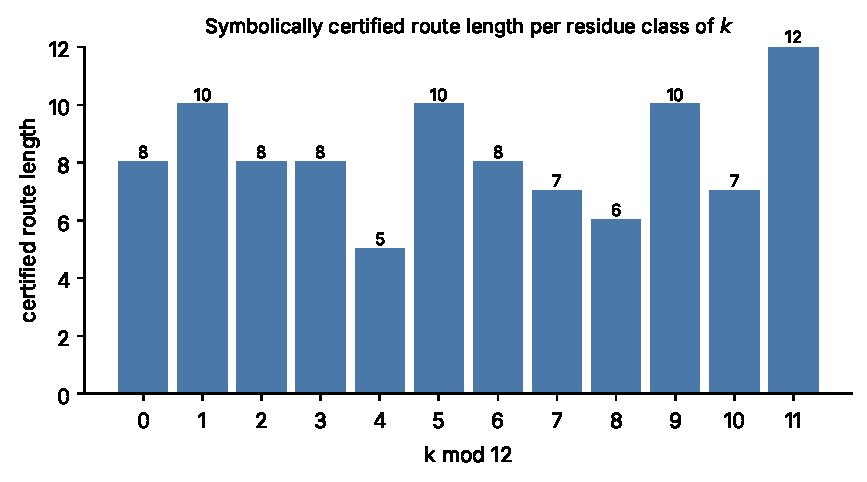
\includegraphics[width=.8\textwidth]{figures/fig1_classes.pdf}
\caption{Length of the certified route for each residue class.}
\end{figure}

\begin{theorem}[all twelve classes]\label{thm:eleven}
For each residue class of $k$ modulo $12$ listed in Table~\ref{tab:classes} there is a route of the stated length from $F_k$ to $F_{k+1}$, valid for all $k\ge20$ in the class. \emph{(Computer-algebra certificate, verifier items S3 and S3b: identities in $O_\varepsilon$; integrality over a full Pisano period; positivity for $b\ge 40$; strict monotonicity of all states.)} As an independent test, every individual step of every route was checked to be an edge of $G$ with the separate predicate \texttt{is\_edge} for all $k<340$ in the class (\NEdgeSteps{} steps; item S4).
\end{theorem}

\begin{figure}[ht]\centering
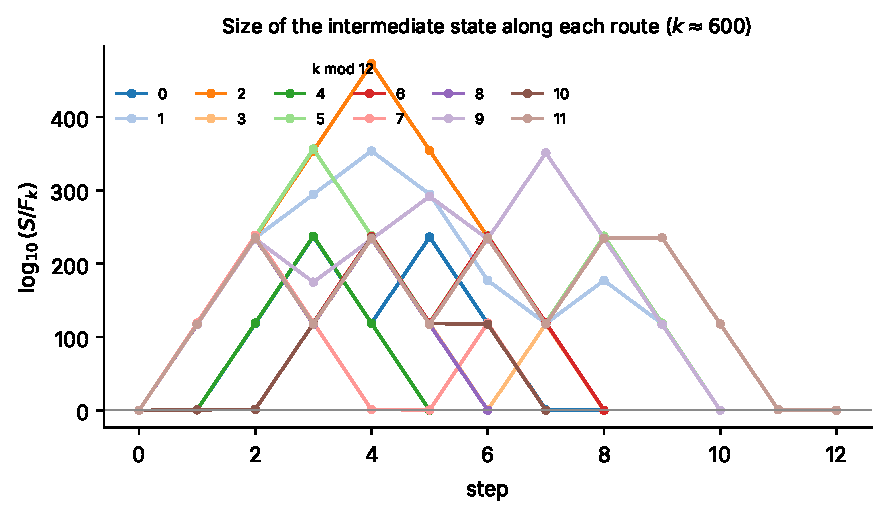
\includegraphics[width=.85\textwidth]{figures/fig2_trajectory.pdf}
\caption{Intermediate states are large: along every route the integer rises to roughly $F_k^{\,2}$--$F_k^{\,5}$ and returns. This is how the routes exploit the squares $(x+1)^2$, $(y+1)^2$.}
\end{figure}

\section{Do the intermediate states determine their parameters?}\label{sec:recover}
A bounded route does not by itself give a restricted selector: the label $N_i$ must be computed from the \emph{current integer} and the finite control state, without access to $k$. We show this is possible for the routes above, under the following explicit reading of R3.

\paragraph{Reading of R3 used.} The allowed inversions are (i) fixed-order integer roots and (ii) inversion by bisection of a function $G(t)$ that is a fixed polynomial in $t$ and $A(t)$, where $A(t)=\lfloor(\isqrt(5t^2+4\varepsilon)-t)/2\rfloor$, provided $G$ is strictly increasing on its domain. For $t=F_h$ one has $A(t)=F_{h-1}$ exactly. Whether this falls under ``a strictly increasing polynomial or a fixed algebraic closed form'' is a matter of reading Definition~2.1; if only a one-variable polynomial is admitted, the statements below do not apply.

\paragraph{Dispatch.} For $x=F_k$ ($k\ge 2$), $5x^2+4(-1)^k=L_k^2$ and $y=F_{k+1}=(x+L_k)/2$. Hence from $x$ alone one computes $L_k$ (testing which of $5x^2\pm4$ is a square) and $y$. The map $k\mapsto(F_k,F_{k+1})\bmod 24$ is injective on a period because the recurrence is invertible, so $(x,y)\bmod 24$ determines $k\bmod 24$, hence the class $k\bmod 12$ and $\varepsilon$.

\begin{proposition}[recovery]\label{prop:rec}
Fix a class and a step $i$ of its route, with state $s_i=p_0(b)+p_1(b)a$. Let $G_i(t)=p_0(t)+p_1(t)A(t)$ for integers $t\ge40$. Then $G_i$ is strictly increasing, $G_i(t)\ge t$, and $G_i(F_h)=s_i$ at the true parameter. Hence $F_h$ is the unique $t\ge 40$ with $G_i(t)=s_i$, and bisection on $[40,s_i]$ finds it.
\end{proposition}
\begin{proof}
$A$ is non-decreasing and integer-valued, since $\isqrt(5t^2+4\varepsilon)$ grows by $2$ or $3$ per unit step. For each state one checks (shifted-coefficient test, item S3b and the monotonicity flag of S3) that $p_1\ge0$ and $p_1'\ge0$ for $t\ge40$ and that $p_0'>0$ and $p_0(t)\ge t$ there. Then $G_i(t+1)-G_i(t)\ge p_0(t+1)-p_0(t)>0$ and $G_i(t)\ge p_0(t)\ge t$.
\end{proof}

\paragraph{Simulation.} A selector was implemented that receives only the integer $F_k$ and keeps only the control pair (class, step): it dispatches, then at each step recovers $b$ by bisection, evaluates $N_i=q_0(b)+q_1(b)A(b)$ exactly, checks legality, and applies the move. For all \NSelTest{} inputs $F_k$ with $30\le k<700$ it ended at $F_{k+1}$ with no failure; the functions $G_i$ were also checked to be strictly increasing on $40\le t<2000$ (item S5). Labels use only $+,-,\times$, division by the constants \DenList{} that occur as coefficient denominators, comparison, and $\isqrt$; no primality test, factorisation, gcd or divisor search occurs. The path part of the control set has \CtlStates{} states, to which come the start state and the finite table for small $k$. The labels in the Appendix are the finite certified list required by R5.

\begin{theorem}[finite-control Fibonacci successor selector]\label{thm:sel}
Under the reading of R3 above, there is a selector satisfying R1--R5, with control set of size \CtlStates{} on the path part plus the start state and an explicit table for $k\le 29$, that on input $F_k$ ($k\ge 2$) outputs a route of at most \MaxLen{} moves ending at $F_{k+1}$.
\end{theorem}
\begin{proof}
For $k\le29$ use the table of Section~\ref{sec:small}. For $k\ge30$ we have $h\ge15$, so $b=F_h\ge 40$ and every state's parameter is recoverable by Proposition~\ref{prop:rec}; dispatch gives the class; the labels $N_i(b)$ are the certified ring elements of Theorem~\ref{thm:eleven}; legality and the endpoint follow from Proposition~\ref{prop:cert}.
\end{proof}
The simulation above is a corroboration of this theorem, not part of its proof; the proof rests on the exact certificates and on Proposition~\ref{prop:rec}.

\section{Small \texorpdfstring{$k$}{k} and the resulting bound}\label{sec:small}
For $2\le k\le 29$ the exact distance $d(F_k,F_{k+1})$ was computed by exhaustive bidirectional search (neighbours enumerated through factorisation), and an explicit path of that length was recorded and re-checked edge by edge with the independent predicate \texttt{is\_edge} (item S6):
\begin{center}\begin{tabular}{@{}lrrrrr@{}}\toprule $d$ & 2 & 3 & 4 & 5 & 6\\\midrule number of $k\in[2,29]$ & 1 & 0 & 3 & 17 & 7\\\bottomrule\end{tabular}
\end{center}
So the certified routes of $5$--$10$ moves are \emph{not} shortest; the true distances are at most \NSmallMax{} for $k\le29$, and we make no claim about their value for larger $k$ beyond the upper bound.

\begin{corollary}\label{cor:bound}
For every $k\ge2$, $d(F_k,F_{k+1})\le\MaxLen$.
\end{corollary}

\paragraph{Caution about interpretation.} In U2-FP v001 ratio-matched non-Fibonacci pairs had a similar distance distribution, so boundedness of $d$ is not special to Fibonacci numbers. What is special here is \emph{uniformity}: one explicit finite list of integer-valued label formulas, proved for infinitely many $k$ at once, with parameters recoverable from the state.

\section{Class 11: how the last route was found}\label{sec:open}
Class $k\equiv 11\pmod{12}$ resisted the full vocabulary. The attempts are listed in \texttt{data/search\_record.json}; in short, with about $1800$ vocabulary values the bidirectional search reached its node cap before the two frontiers met at depth $10$ (modulus $12$; and, separately, moduli $24$ with $r=11$ and $r=23$) and at depth $12$ with three million nodes. Reducing the vocabulary to the $1536$ values with small coefficients (linear forms with $|u|,|v|\le2$, $|w|\le1$, denominators $1,2,4$, all products $\lambda PQ$, the small constants) lowered the branching factor, and the same search met after about $1070$\,s at total depth $12$ (six moves from each side). The candidate replayed correctly on $122$ values of $k$ and was then certified like the others. Two lessons: the obstacle was the branching factor, not the expressiveness of the vocabulary; and the route has $12$ moves although the exact distance for $k=11$ and $k=23$ is $5$ and $6$, so a considerably shorter route for this class very probably exists.

\section{Conclusions and next steps}
(1) The three families of UNNS-U2-FP v001 are now proved. (2) The nine remaining classes now have certified routes, so all \NCov{} residue classes of $k$ are covered, with routes of at most \MaxLen{} moves. (3) Intermediate states determine their parameters under the reading of R3 given above, and the pieces assemble into a finite-control Fibonacci successor selector (Theorem~\ref{thm:sel}). (4) The decisive remaining tasks are: settle whether the reading of R3 in Section~\ref{sec:recover} is acceptable, or replace the bisection by inversion of a one-variable polynomial; search for shorter routes (the certified lengths $5$--$12$ exceed the exact distances $2$--$6$ found for $k\le29$); and re-verify the exact certificates in a proof assistant. Prime generation remains a separate open problem.

\begin{thebibliography}{9}
\bibitem{sympy} A.~Meurer et al., SymPy: symbolic computing in Python, \emph{PeerJ Computer Science} \textbf{3}:e103 (2017).
\bibitem{wall} D.~D.~Wall, Fibonacci series modulo $m$, \emph{Amer.\ Math.\ Monthly} \textbf{67} (1960), 525--532.
\bibitem{vajda} S.~Vajda, \emph{Fibonacci and Lucas Numbers, and the Golden Section}, Ellis Horwood, 1989.
\bibitem{fp} UNNS Research Collective, UNNS-U2-FP v001 (frozen); with U1-BND v001, U2-001 v001, U2-SQ v001.
\end{thebibliography}

\appendix
\section{Route labels}
Labels as found by the search; $F_j,L_j$ with $h=\lfloor k/2\rfloor$. Moves $1,\dots,n_f$ are read forward from $F_k$ with $S$ the state before the move; the later moves were found from the $F_{k+1}$ side, and there $S$ is the state \emph{after} the move. The ring-element form of every $N_i$ and $s_i$ is in \texttt{data/class\_certificates.json}.
\small\renewcommand{\arraystretch}{1.35}
\begin{minipage}{\linewidth}\noindent\textbf{Class $k\equiv 0 \pmod{12}$.}\\[1pt]
\begin{tabular}{@{\hspace{1.5em}}rcl@{}}
1 & $+$ & $N=1$\\
2 & $+$ & $N=S/4$\\
3 & $+$ & $N=S/F_{h-1}^2$\\
4 & $-$ & $N=4F_hF_{h+2}$\\
5 & $+$ & $N=F_{h+1}^2-1$\\
6 & $-$ & $N=-x+2y+2$\\
7 & $-$ & $N=S/4$\\
8 & $-$ & $N=1$\\
\end{tabular}\end{minipage}\par\medskip
\begin{minipage}{\linewidth}\noindent\textbf{Class $k\equiv 1 \pmod{12}$.}\\[1pt]
\begin{tabular}{@{\hspace{1.5em}}rcl@{}}
1 & $+$ & $N=S$\\
2 & $+$ & $N=S/\left(3x-y+2\right)$\\
3 & $+$ & $N=2F_{h-1}+3F_h$\\
4 & $+$ & $N=2F_{h-1}+3F_h+1$\\
5 & $-$ & $N=\dfrac{2F_{h-1}+3F_h+2}{2}-1$\\
6 & $-$ & $N=F_{h+1}^2$\\
7 & $-$ & $N=F_{h-1}+F_h-1$\\
8 & $+$ & $N=\dfrac{F_{h-1}+2F_h+1}{2}-1$\\
9 & $-$ & $N=F_{h-1}+2F_h$\\
10 & $-$ & $N=S$\\
\end{tabular}\end{minipage}\par\medskip
\begin{minipage}{\linewidth}\noindent\textbf{Class $k\equiv 2 \pmod{12}$.}\\[1pt]
\begin{tabular}{@{\hspace{1.5em}}rcl@{}}
1 & $+$ & $N=S$\\
2 & $+$ & $N=F_{h+1}^2$\\
3 & $+$ & $N=\dfrac{-2x+2y+2}{2}$\\
4 & $+$ & $N=4L_{h+1}L_{h-1}$\\
5 & $-$ & $N=4F_h^2$\\
6 & $-$ & $N=L_{h-1}^2$\\
7 & $-$ & $N=y+1$\\
8 & $-$ & $N=S$\\
\end{tabular}\end{minipage}\par\medskip
\begin{minipage}{\linewidth}\noindent\textbf{Class $k\equiv 3 \pmod{12}$.}\\[1pt]
\begin{tabular}{@{\hspace{1.5em}}rcl@{}}
1 & $+$ & $N=S$\\
2 & $+$ & $N=2x+y+2$\\
3 & $-$ & $N=F_h^2-1$\\
4 & $+$ & $N=4F_{h-1}F_{h+1}$\\
5 & $-$ & $N=4L_h^2$\\
6 & $-$ & $N=S/4$\\
7 & $+$ & $N=\sqrt{S/\left(12\right)}-1$\\
8 & $-$ & $N=S/3$\\
\end{tabular}\end{minipage}\par\medskip
\begin{minipage}{\linewidth}\noindent\textbf{Class $k\equiv 4 \pmod{12}$.}\\[1pt]
\begin{tabular}{@{\hspace{1.5em}}rcl@{}}
1 & $+$ & $N=1$\\
2 & $+$ & $N=S/4$\\
3 & $+$ & $N=\dfrac{x+3y+2}{4}-1$\\
4 & $-$ & $N=-x+2y+2$\\
5 & $-$ & $N=S$\\
\end{tabular}\end{minipage}\par\medskip
\begin{minipage}{\linewidth}\noindent\textbf{Class $k\equiv 5 \pmod{12}$.}\\[1pt]
\begin{tabular}{@{\hspace{1.5em}}rcl@{}}
1 & $+$ & $N=S$\\
2 & $+$ & $N=3x-y+2$\\
3 & $+$ & $N=2x+y+2$\\
4 & $-$ & $N=F_{h-1}F_{h+1}-1$\\
5 & $-$ & $N=y-2$\\
6 & $+$ & $N=\dfrac{y}{2}-1$\\
7 & $-$ & $N=\dfrac{-x+2y-1}{2}$\\
8 & $+$ & $N=F_{h-1}F_{h+2}-1$\\
9 & $-$ & $N=3x-y+2$\\
10 & $-$ & $N=S$\\
\end{tabular}\end{minipage}\par\medskip
\begin{minipage}{\linewidth}\noindent\textbf{Class $k\equiv 6 \pmod{12}$.}\\[1pt]
\begin{tabular}{@{\hspace{1.5em}}rcl@{}}
1 & $+$ & $N=S$\\
2 & $+$ & $N=F_{h+1}^2$\\
3 & $-$ & $N=\dfrac{-2x+2y+2}{4}-1$\\
4 & $+$ & $N=\dfrac{-2x+2y-2}{8}$\\
5 & $-$ & $N=\dfrac{-2x+2y+2}{4}$\\
6 & $+$ & $N=-x+y+1$\\
7 & $-$ & $N=S/\left(x+3y+2\right)$\\
8 & $-$ & $N=S$\\
\end{tabular}\end{minipage}\par\medskip
\begin{minipage}{\linewidth}\noindent\textbf{Class $k\equiv 7 \pmod{12}$.}\\[1pt]
\begin{tabular}{@{\hspace{1.5em}}rcl@{}}
1 & $+$ & $N=S$\\
2 & $+$ & $N=2x+y+2$\\
3 & $-$ & $N=\dfrac{3x-y+2}{4}-1$\\
4 & $-$ & $N=\dfrac{y-1}{2}-1$\\
5 & $-$ & $N=1$\\
6 & $+$ & $N=\sqrt{S/\left(12\right)}-1$\\
7 & $-$ & $N=S/3$\\
\end{tabular}\end{minipage}\par\medskip
\begin{minipage}{\linewidth}\noindent\textbf{Class $k\equiv 8 \pmod{12}$.}\\[1pt]
\begin{tabular}{@{\hspace{1.5em}}rcl@{}}
1 & $+$ & $N=S$\\
2 & $+$ & $N=4L_{h+1}^2$\\
3 & $-$ & $N=4F_hF_{h+2}$\\
4 & $+$ & $N=F_{h+1}^2-1$\\
5 & $-$ & $N=-x+2y+2$\\
6 & $-$ & $N=S$\\
\end{tabular}\end{minipage}\par\medskip
\begin{minipage}{\linewidth}\noindent\textbf{Class $k\equiv 9 \pmod{12}$.}\\[1pt]
\begin{tabular}{@{\hspace{1.5em}}rcl@{}}
1 & $+$ & $N=S$\\
2 & $+$ & $N=S/\left(3x-y+2\right)$\\
3 & $-$ & $N=2F_{h-1}+3F_h-1$\\
4 & $+$ & $N=\dfrac{2F_{h-1}+3F_h-1}{2}$\\
5 & $+$ & $N=\dfrac{2F_{h-1}+3F_h+1}{2}$\\
6 & $-$ & $N=\dfrac{2F_{h-1}+3F_h-1}{4}$\\
7 & $+$ & $N=F_{h+3}^2-1$\\
8 & $-$ & $N=F_{h+1}^2$\\
9 & $-$ & $N=S/\left(3x-y+2\right)$\\
10 & $-$ & $N=S$\\
\end{tabular}\end{minipage}\par\medskip
\begin{minipage}{\linewidth}\noindent\textbf{Class $k\equiv 10 \pmod{12}$.}\\[1pt]
\begin{tabular}{@{\hspace{1.5em}}rcl@{}}
1 & $+$ & $N=1$\\
2 & $+$ & $N=4$\\
3 & $+$ & $N=x$\\
4 & $+$ & $N=\dfrac{x+3y-2}{4}$\\
5 & $-$ & $N=-x+2y+2$\\
6 & $-$ & $N=4$\\
7 & $-$ & $N=S$\\
\end{tabular}\end{minipage}\par\medskip
\begin{minipage}{\linewidth}\noindent\textbf{Class $k\equiv 11 \pmod{12}$.}\\[1pt]
\begin{tabular}{@{\hspace{1.5em}}rcl@{}}
1 & $+$ & $N=S$\\
2 & $+$ & $N=S/F_h^2$\\
3 & $-$ & $N=\sqrt{S/\left(F_{h+2}^2\right)}-1$\\
4 & $+$ & $N=S/\left(4F_{h+2}^2\right)$\\
5 & $-$ & $N=\sqrt{S/\left(F_{h+2}^2\right)}-1$\\
6 & $+$ & $N=F_{h+2}^2$\\
7 & $-$ & $N=S/\left(2L_{h+1}L_{h-1}\right)$\\
8 & $+$ & $N=\sqrt{S/\left(4L_{h-1}F_{h+3}\right)}-1$\\
9 & $+$ & $N=3$\\
10 & $-$ & $N=L_{h-1}F_{h+3}$\\
11 & $-$ & $N=S/12$\\
12 & $-$ & $N=1$\\
\end{tabular}\end{minipage}\par\medskip

\end{document}
